%%%%%%%%%%%%%%%%%%%%%%%%%%%%%%%%%%%%%%%%%%%%%%%%%%%%%%%%%%%%%%%%%%%%%
%%%
%%% Set these variables appropriately
%%%
\newcommand{\AUTHORS}{Justin Athill, Angela Hillsman, and Daniel Wood}
\newcommand{\TITLE}{PAPER TITLE HERE}
\newcommand{\KEYWORDS}{}
\newcommand{\CONFERENCE}{}
\newcommand{\PAGENUMBERS}{yes}       % "yes" or "no"
\newcommand{\TOAPPEAR}{no}
%%%
%%%
%%%%%%%%%%%%%%%%%%%%%%%%%%%%%%%%%%%%%%%%%%%%%%%%%%%%%%%%%%%%%%%%%%%%%

%%%% Setup the document/page
\documentclass[pdftex,twoside,twocolumn,11pt,letterpaper]{article}
\usepackage{ifthen}

\ifthenelse{\equal{\PAGENUMBERS}{yes}}{%
\usepackage[nohead,
            left=1in,right=1in,top=1in,
            footskip=0.5in,bottom=0.75in     % Room for page numbers
            ]{geometry}
}{%
\usepackage[noheadfoot,columnsep=0.2in,
            margin=1in,centering,truedimen]{geometry}
}

\usepackage{fancyhdr}
\usepackage[numbers,sort]{natbib}
\usepackage{xspace}
\usepackage{booktabs}
\usepackage{subfigure}
\usepackage[T1]{fontenc}
\usepackage{textcomp}
\usepackage{mathptmx}   % Times + Times-like math symbols
\usepackage{courier}
\usepackage[scaled=0.92]{helvet}

\usepackage{color}
\usepackage[pdftex]{graphicx}
\ifthenelse{\isundefined{\wantBW}}{%
  \usepackage[colorlinks]{hyperref}%        % for online version
}{%
  \usepackage[pdfborder={0 0 0}]{hyperref}% % for paper (B&W) version
}
\newcommand{\URL}[1]{\url{#1}}

%%%%% Setup for PDF
\hypersetup{%
pdfauthor = {\AUTHORS},
pdftitle = {\TITLE},
pdfsubject = {\CONFERENCE},
pdfkeywords = {\KEYWORDS},
bookmarksopen = {true}
}

%\setlength{\parindent}{0pt}
%\setlength{\parskip}{0pt}
\renewcommand{\headrulewidth}{0pt}
\newcommand{\Paragraph}[1]{\vspace{-2ex}\paragraph{#1.}}
\setlength{\topmargin}{-.15in}

\ifthenelse{\equal{\PAGENUMBERS}{yes}}{%
  \pagestyle{plain}
}{%
  \pagestyle{empty}
}

\makeatletter\long\def\@makecaption#1#2{
   \vskip 10pt
   \setbox\@tempboxa\hbox{\textsf{#1: #2}}
   \ifdim \wd\@tempboxa >\hsize % IF longer than one line:
       \textsf{#1: #2}\par      % THEN set as ordinary paragraph.
     \else                      % ELSE  center.
       \hbox to\hsize{\hfil\box\@tempboxa\hfil}
   \fi}
\makeatother

\clubpenalty=10000  % Don't allow orphans
\widowpenalty=10000 % Don't allow widows

\title{\textbf{\TITLE}}
\author{\AUTHORS}
\date{}

% Compact itemize and enumerate.  Note that they use the same counters and
% symbols as the usual itemize and enumerate environments.
\def\compactify{\itemsep=0pt \topsep=0pt \partopsep=0pt \parsep=0pt}
\let\latexusecounter=\usecounter
\newenvironment{CompactItemize}
  {\def\usecounter{\compactify\latexusecounter}
   \begin{itemize}}
  {\end{itemize}\let\usecounter=\latexusecounter}
\newenvironment{CompactEnumerate}
  {\def\usecounter{\compactify\latexusecounter}
   \begin{enumerate}}
  {\end{enumerate}\let\usecounter=\latexusecounter}

\newcommand{\comment}[1]{\textcolor{red}{#1}}
\newcommand{\ignore}[1]{}

\newcommand{\xc}[1]{\mbox{\textit{#1}}}
\newcommand{\la}{\leftarrow}
\newcommand{\ra}{\rightarrow}
\newcommand{\somespace}{\hspace{0.1cm}}

\def\discretionaryslash{\discretionary{/}{}{/}}
\def\discretionarydot{\discretionary{.}{}{.}}
\def\discretionarycolon{\discretionary{:}{}{:}}
{\catcode`\/\active
\catcode`\.\active
\catcode`\:\active
\gdef\URLprepare{\catcode`\/\active\let/\discretionaryslash
                 \catcode`\.\active\let.\discretionarydot
                 \catcode`\:\active\let:\discretionarycolon
        \def~{\char`\~}}}%
\def\URL{\bgroup\URLprepare\realURL}%
\def\realURL#1{\tt #1\egroup}%

\newcommand{\eg}{{\em e.g.}, }
\newcommand{\ie}{{\em i.e.}, }
\newcommand{\etal}{{\em et al.\ }}

\def\check{\stackrel{{\scriptscriptstyle ?}}{=}}

\begin{document}
\maketitle

% -*-LaTeX-*-
% $Id: abstract.tex 70 2007-01-30 21:59:16Z nicolosi $

\begin{abstract}
ABSTRACT HERE
\end{abstract}

   
\section{Introduction}
\label{sec:intro}
The Heavy Hitter problem refers to the objective of identifying the heaviest flows in a stream of data. In one variant of the problem, heavy flows are classified as those with a frequency above a threshold t. In this paper, we address a second variant of the problem--``top-k.'' In this variant, the heavy hitters are the top k flows by frequency. 

There are many potential flows that can be analyzed in the context of the Heavy Hitters problem, including source IP addresses, destination IP addresses, transport port numbers, or five-tuples. Depending on the application of the algorithm, a different conception of flow may be appropriate. In this case, we employ the Heavy Hitters algorithm for DoS detection by identifying hosts that are responsible for sending the most traffic through an ISP link. Due to the nature of Internet traffic, a relatively few number of hosts are responsible for sending the majority of packets through a network. In fact, the top 3 percent of hosts may account for over half of packets traveling through an ISP link in a given time period. Figure 1, a graph of cumulative traffic addressed to/from the top k sources/destinations, reveals two important conclusions about the distribution of traffic. First, there are approximately twice as many destinations as sources, and as a result, these sources account for more traffic on average. Second, for both source addresses and destination addresses, the heaviest hitters are responsible for a highly disproportionate amount of network traffic. Through the rest of this paper, we consider the frequency of packets identified by source IP address as our measure of heavy hitters.

\begin{figure}[t]
  \centering
    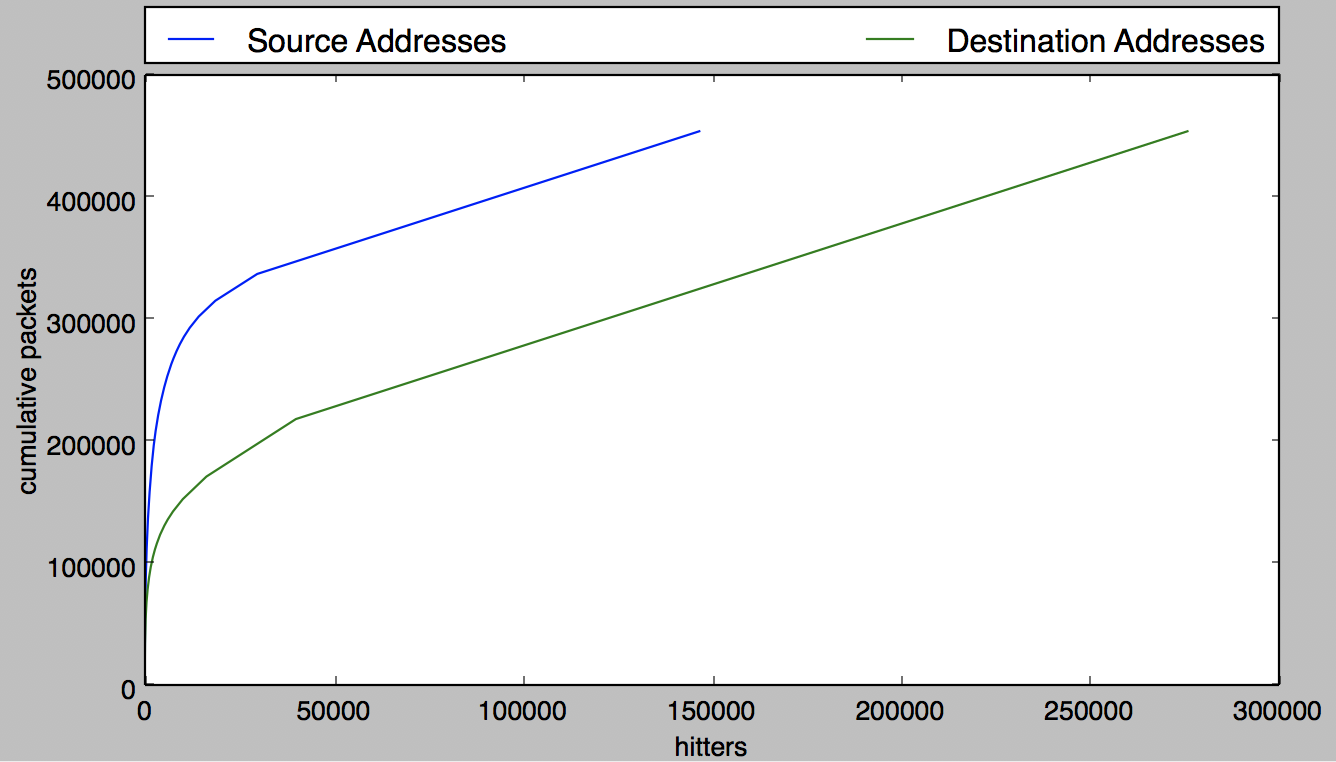
\includegraphics[scale=0.3]{cumulative}
     \caption{Graph of the cumulative traffic addressed to/from the top k sources/destinations, captured from an ISP backbone link}
     \label{fig:bp-image}
\end{figure}

\section{Design}
\label{sec:design}
\subsection{Probabilistic Minimum}
Starting with the Space Saving algorithm as a baseline, we first settled on probabilistic sampling as a way to make finding the minimum element more efficient, rather than linearly searching the entire table. As long as a flow with a low enough frequency is evicted when a new flow is encountered, larger flows will still be preserved in the table. As Figure~\ref{fig:probMin} shows, sampling as few as 4 elements probabilistically ensures that only elements in the lowest quintile will be evicted. Drawing from HashPipe, we implemented this optimization using a hash table pipeline, as the number of stages equals the number of elements probabilistically sampled. If there are four stages in the pipeline, the minimum of the four flows encountered will be a candidate for eviction. 
\begin{figure}[t]
  \centering
    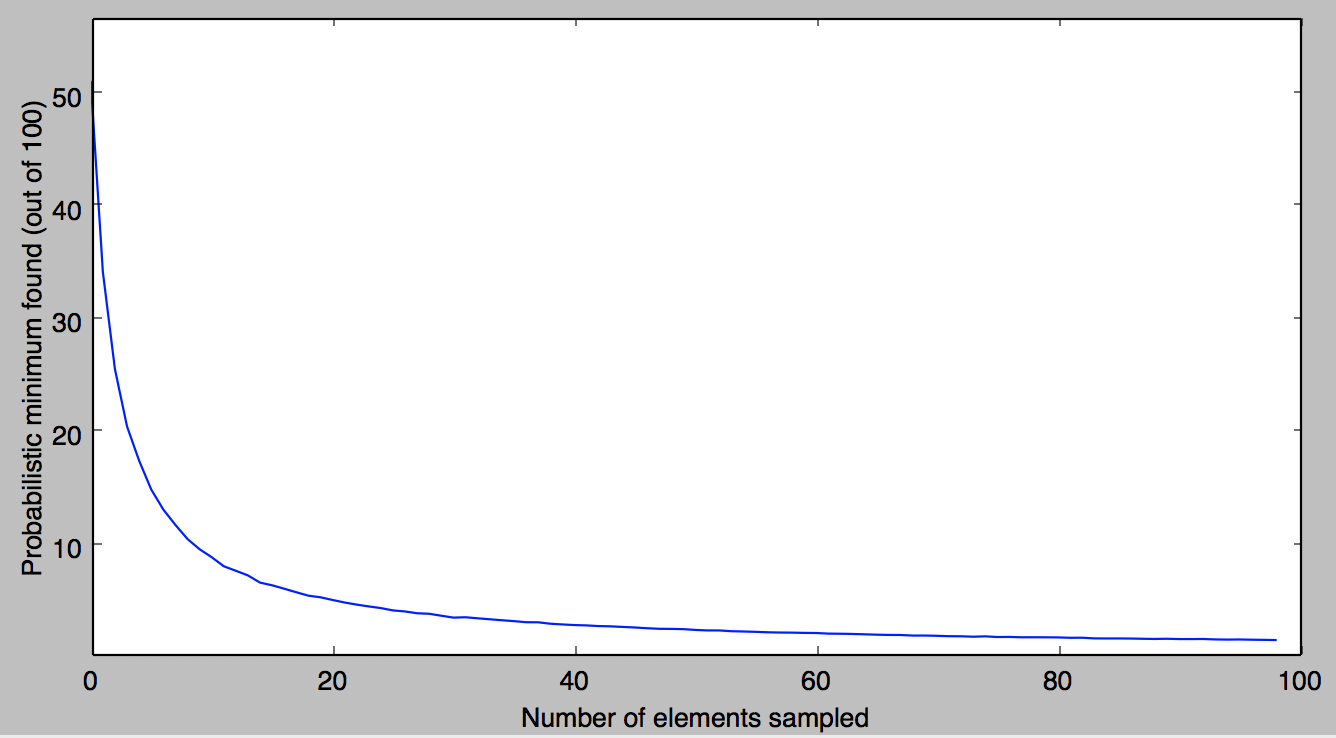
\includegraphics[scale=0.32]{probMin}
     \caption{The minimum of a randomly selected set of elements approaches the true minimum.}
     \label{fig:probMin}
\end{figure}
\subsection{Randomized Assignment}
HashPipe, as the name suggests, features a consistent hashing scheme whereby each stage uses an independent hash function and subsequent repeated flows consistently hash to the same location within each stage. This scheme is intended to reduce the number of duplicate flows occupying space in the pipeline and consolidate their counts. However, we experimentally determined that using a random function to determine flow assignment within the first stage resulted in improvements in accuracy of nearly 50 percent.
\subsection{Logarithmic Admission Policy}
One of the major flaws with HashPipe is the fact that, as with Space Saving, every flow will always be admitted into the pipeline, even if it will never reoccur. In streams with many small flows, accuracy suffers as heavy hitters near the minimum threshold are evicted by small newly encountered flows. Therefore, in HashFilter, we introduced a modified admission policy inspired by RAP, but instead of making the probability of admission inversely proportional to the frequency of the minimum counter, we used a log function to dampen extremely low admission probabilities. We introduced a log function to counteract one of the systematic errors with RAP: denying admission to new heavy hitters. This way, flows with high frequencies are still protected, but smaller flows have a larger probability of being evicted. We tested two potential solutions to this problem, both of which restrict admission to the table. We call these variants of HashFilter Front Rejection and Back Rejection. Our implementation can be accessed at \verb+github.com/danielwood95/heavyHitters+

In Front Rejection (A.K.A. The Bouncer), packets are randomly assigned a slot in the first stage. If empty, the packet is inserted and the frequency is set to 1. If the slot contains a packet with the identical source IP address, the frequency is incremented. Otherwise, the packet evicts the resident of the slot with probability $p = 1 / (5*log(c_m + 1))$, where $c_m$ is the frequency count of the flow in the slot. This is easy to implement, and it saves a lot of computational resources further down the pipeline, since on average 90 percent of packets will be refused admission to the pipeline. However, it is not necessarily accurate because the probability of admission is determined by only the flow randomly compared to in the first stage of the pipeline. This flow is not guaranteed to the be the minimum, but it is likely to be an average flow, which turns out to be an adequate compromise. The pseudo code is detailed in Algorithm 3. 

In Back Rejection (A.K.A. The Interview), all packets are admitted to the entrance of the pipeline and proceed through all stages of the pipeline. However, rather than always evicting the minimum of the flows encountered throughout the pipeline to make way for the new flow, a calculation is made at the end of the pipeline. With probability $p = 1 / (5*log(c_m + 1))$, the minimum flow is evicted, otherwise the minimum flow is inserted back into the first stage, retroactively denying admission to the newly encountered flow located in the first stage. 
\begin{figure}[t]
  \centering
    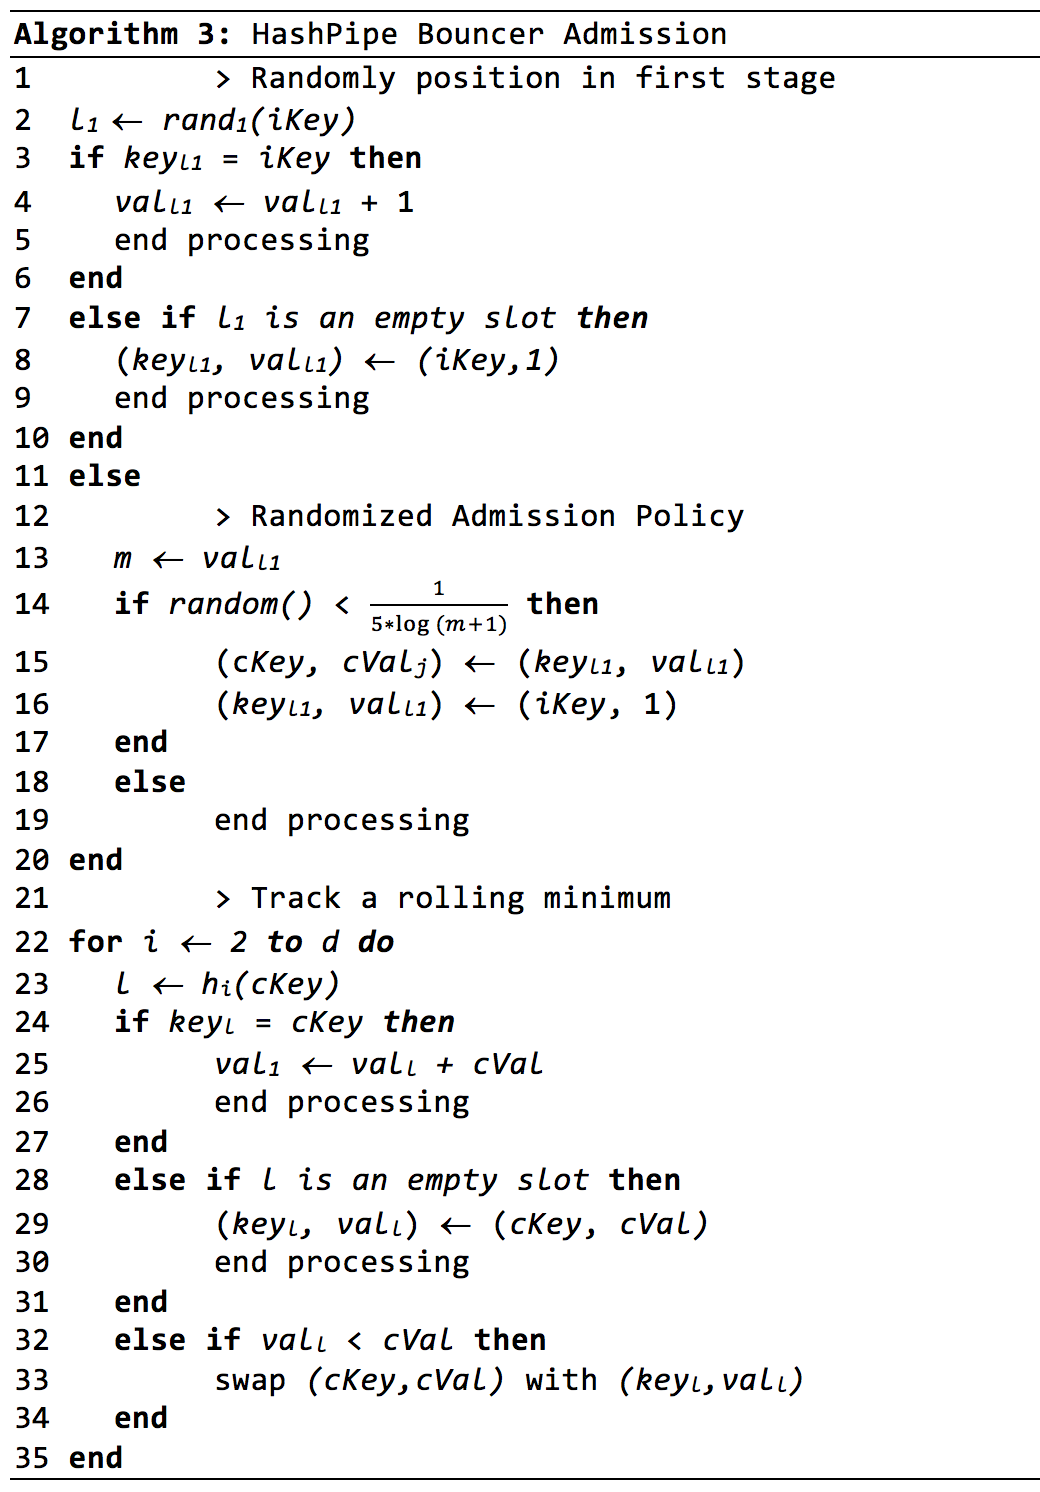
\includegraphics[scale=0.42]{alg3}
     \label{fig:bp-image}
\end{figure}
\section{Evaluation}
\label{sec:eval}

We evaluate the accuracy of the variants of our algorithm through a series of simulations in which we fine tune the various parameters: number of stages, memory size, and randomized admission policy coefficients. In order to simulate realistic streams of traffic, we ran testing using three different traces from the equinox chicago ISP backbone link, recorded in 2016. These anonymized traces each contain between 20 - 40 million packets, over 1 million different flows, and range from 40 minutes to 1 hour long. The data was obtained with permission from the Center for Applied Internet Data Analysis (CAIDA). We parsed the data from the CAIDA traces to isolate only the source IP addresses. Each source IP address is considered a separate flow.

\subsection{Accuracy Metrics}
Through measuring the false negative rate when testing our algorithms against the CAIDA data, we attempted to experimentally determine which combination of design policies yielded the best results. We focused on testing the two different admission policies, and applied different levels of randomized ``hashing'' to find an optimal algorithm. When applying front rejection, we found that uniformly randomizing the table index in the first stage only yielded the best results, and gave as much as a 50 percent accuracy improvement over simple front rejection with normal hashing (see Figure X). While some randomization provided improvements for front rejection, our tests of back rejection showed that normal hashing at all stages was best (see Figure X).

Why is there a discrepancy in the effectiveness of random hashing? Perhaps this can be explained by the increased level of eviction that occurs in the first stage when random indices are used. When hashes are randomized, it is less likely that the same key will end up at the same index and increase its count in the first stage. So effectively, keys are more quickly pushed to later stages where there is a greater emphasis on retaining heavy flows. Since consistent hashing is performed in later stages, the same key is able to add to its count, and can do this more frequently when it is quickly sent down the pipeline from the first stage. Randomized hashing more effectively treats the first stage as transient, so light flows will more quickly be evicted and heavy flows will more quickly be retained in the core of the pipeline. For this reason, randomizing indices in all stages is less effective because retention also is lower in the latter stages, when it is most important to hold onto heavy flows. Randomization in the first stage adds an accuracy boost to front rejection, but it introduces problems with the more complex back rejection policy. The goal with the Interview policy, is to deny first stage admission to the incoming key at a high rate, and replace it with the probabilistic minimum that emerges from the pipeline. However, when randomization is applied, we can't guarantee that we are swapping the minimum with the incoming key in the first stage. This renders our stricter admission policy ineffective if we can't guarantee that the incoming key is the one being evicted in the first stage. Evidently, randomized hashing  in the first stage can effectively increase accuracy under the right conditions, and was even shown to be useful as a standalone improvement to HashPipe without applying front or back rejection (see Figure X). However, front rejection does not benefit from randomized hashing, and the standalone version of the policy ended up with the best performance.

We were also able to tune our algorithm's performance by experimenting with the multiplicative factor in our logarithmic admission equation. Figure X shows how performance was best at values between 1 and 10, so we settled on a factor of 5 for all future experimentation.



\subsection{Comparison of HashPipe Implementations}
We began algorithm comparison by varying the available memory size, which corresponds to a greater number of counters that can be stored across all hash tables. Figure 2 shows our results when searching for the top 300 flows and using 6 table stages. Both algorithms that applied an admission policy outperformed the standard HashPipe algorithm for all tested memory sizes. Accuracy rates improved by about 20 percent when the number of counters was limited to 300, equal to the number of flows top-k flows being identified, and increases to more than 50 percent improvement when more than 2000 counters are used. HashPipe with front rejection in particular brought its accuracy rate to more than 90 percent with 2000 counters, which is less than half the memory required by the standard HashPipe algorithm to achieve that accuracy with 300 heavy hitters and 6 table stages. In all algorithms, improvement begins to diminish after 1000 counters are available.

In addition to testing the impact of varying memory, we also experimented with the number of table stages available. HashPipe tends to perform best with a limited amount of stages so that the number of duplicates is limited. The optimal number of stages is about 6 with the standard HashPipe, but Figure 3 shows that our algorithms continue to improve past this point as the number of table stages is increased. While Interview and Bouncer also experience diminishing returns after about 8 table stages, they do not see the same performance decrease present in the standard HashPipe algorithm.

\subsection{Space Saver Comparison}
As a final benchmark, we compare our algorithms to the Space Saver algorithm, which finds the true minimum of all of its counters. While this algorithm allows for more accuracy, hardware constraints that restrict multiple reads to the same table make implementations of this algorithm unrealistic. Figure X shows that our algorithms fall behind an idealized implementation of Space Saver, where it is no issue to compute a global minimum. Similar to the baseline implementation of HashPipe, our implementations also outperform Space Saver when a low amount of memory is available. This is because Space Saver is only guaranteed to hold onto the kth heaviest item when it is larger than average count in the table, so its full benefits are realized when memory is increased


\begin{figure}[t]
  \centering
    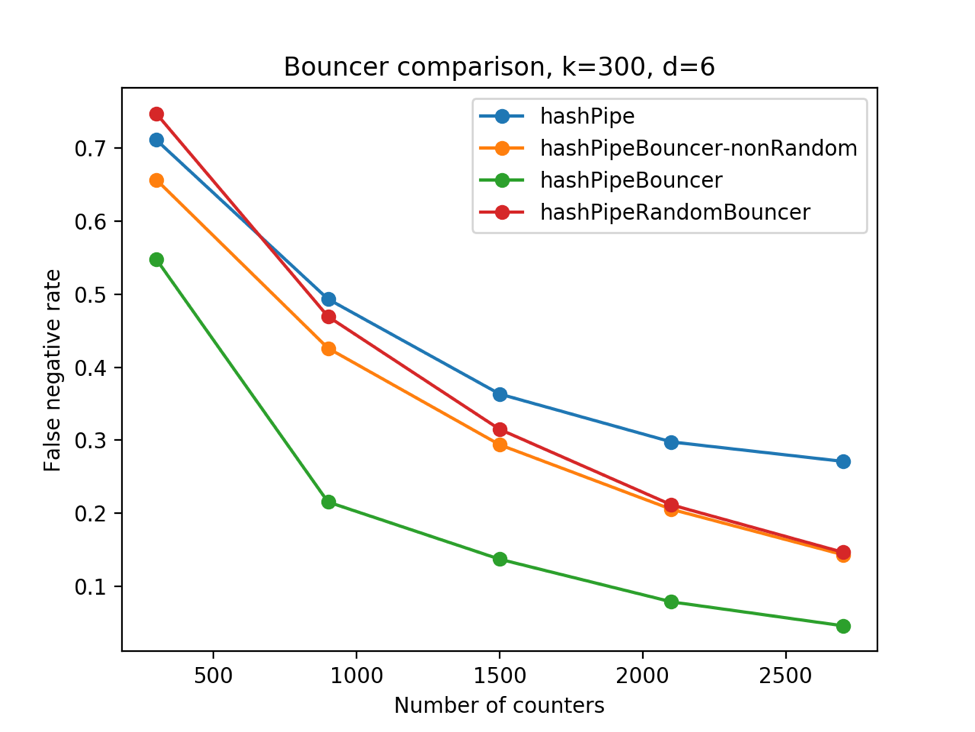
\includegraphics[scale=0.5]{bouncer}
     \caption{Comparison of Bouncer admission policy algorithm with different levels of random hashing. In hashPipeBouncer-nonRandom, consistent hash functions are used in every stage, and no randomnes is applied. The hashPipeBouncer algorithm, only applies randomness in the first stage--should an incoming packet be admitted to the table, it is placed at a random index rather than using a hash function. This variation performed the best across all tested memory sizes and is the main Bouncer algorithm we use in further comparison. The hashPipeRandomBouncer algorithm does comparisons and inserts at random indices in all table stages, and was also shown to be outperformed by limiting randomization to the first stage.}
     \label{fig:bp-image}
\end{figure}

\begin{figure}[t]
  \centering
    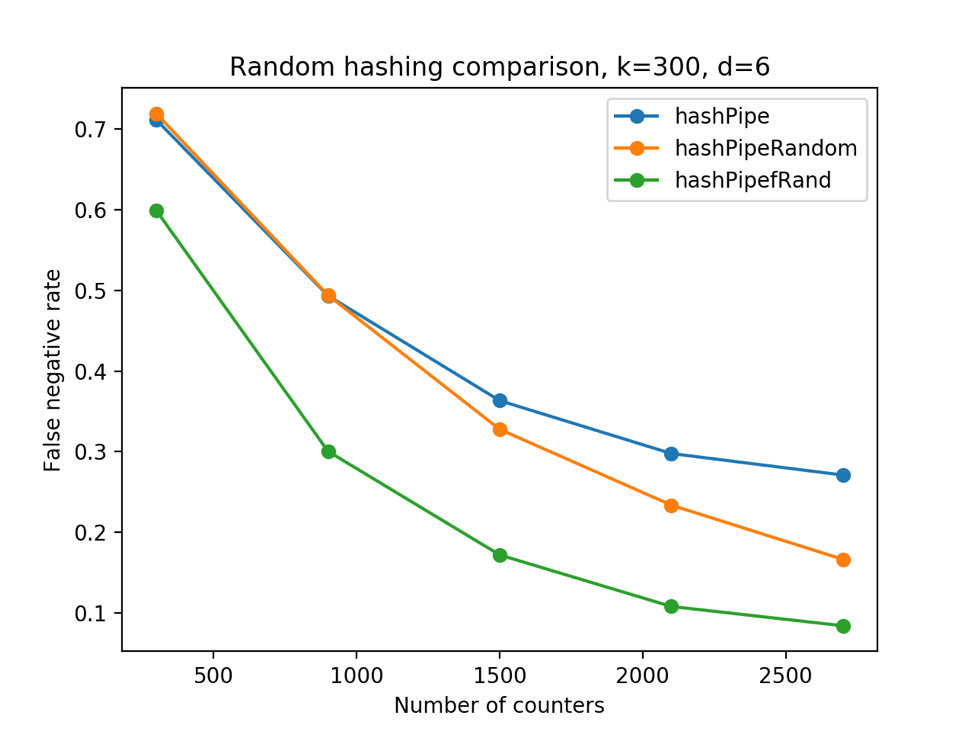
\includegraphics[scale=0.5]{interview}
     \caption{Impact of random hashing rather than using hash functions. The hashPipeRandom algorithm randomizing indices in all stages and provides some benefits at high memory sizes. The hashPipefRand algorithm only hashes to a random index in the first stage and then uses consistent hash functions in the following stages. Randomization in the first stage improves accuracy rates across the entire tested memory range, showing that randomization is useful absent any strict admission policy.}
\end{figure}

\begin{figure}[t]
  \centering
    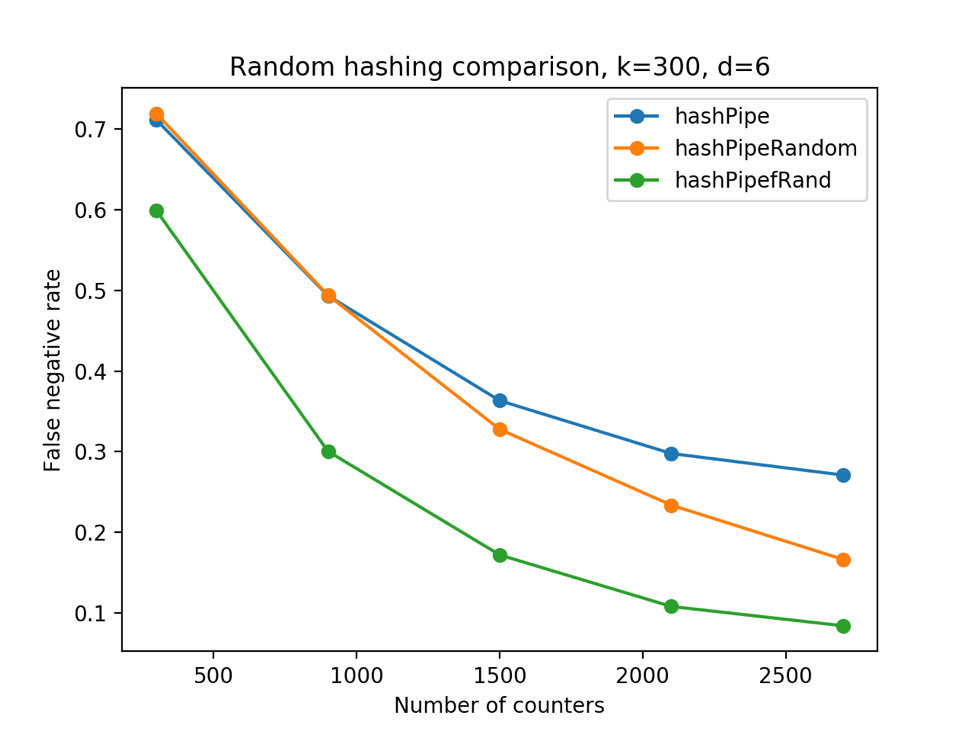
\includegraphics[scale=0.5]{random}
     \caption{Impact of random hashing rather than using hash functions. The hashPipeRandom algorithm randomizing indices in all stages and provides some benefits at high memory sizes. The hashPipefRand algorithm only hashes to a random index in the first stage and then uses consistent hash functions in the following stages. Randomization in the first stage improves accuracy rates across the entire tested memory range, showing that randomization is useful absent any strict admission policy.}
     \label{fig:bp-image}
\end{figure}

\begin{figure}[t]
  \centering
    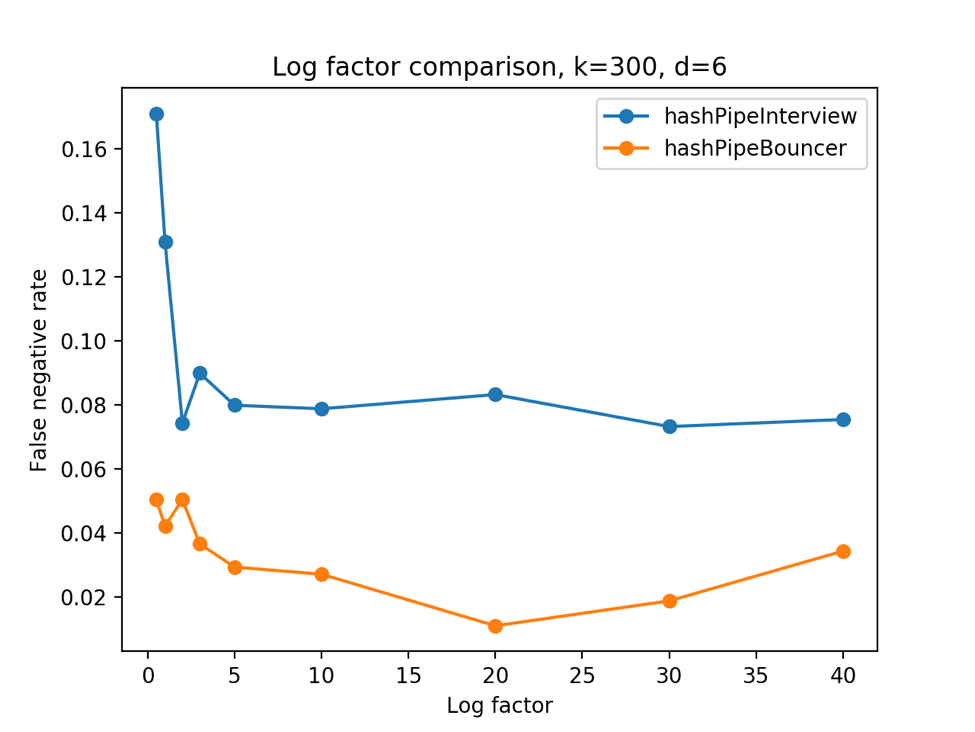
\includegraphics[scale=0.5]{log}
     \caption{Impact of varying the factor f when calculating the admission threshold $p = 1 / (f*log(c_m + 1))$. Results show that factors of 5 and greater experienced relatively similar accuracy rates for both front rejection and back rejection.}
     \label{fig:bp-image}
\end{figure}

\begin{figure}[t]
  \centering
    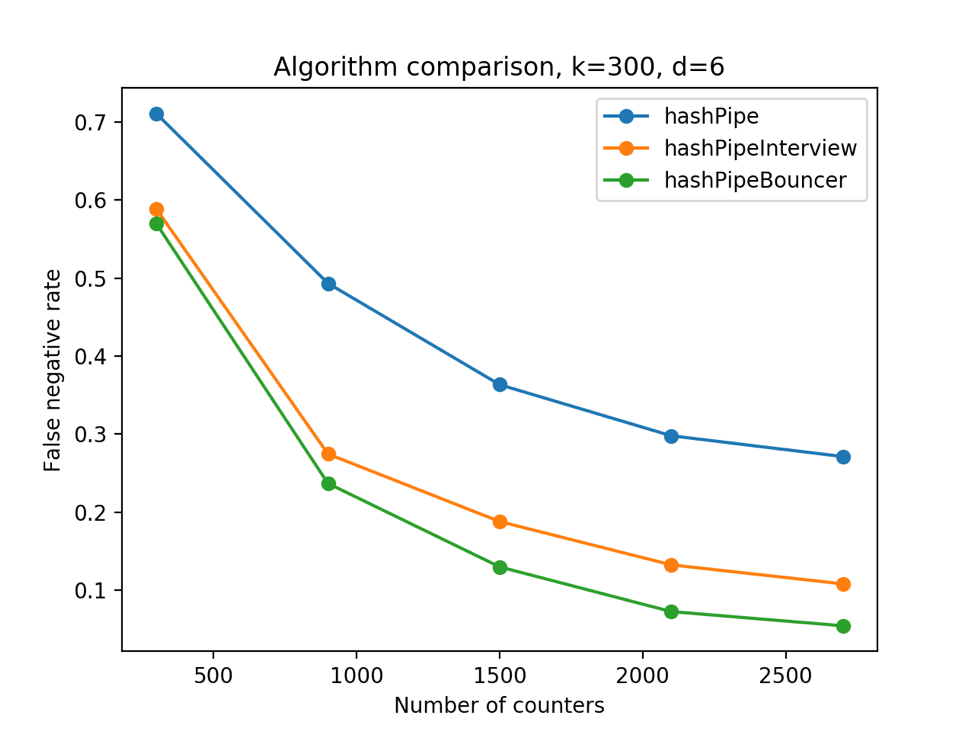
\includegraphics[scale=0.5]{falsenegatives}
     \caption{Comparison of false negatives of Interview and Bouncer to baseline. Both algorithm optimizations improve on the standard HashPipe algorithm over the entire tested memory range}
     \label{fig:bp-image}
\end{figure}

\begin{figure}[t]
  \centering
    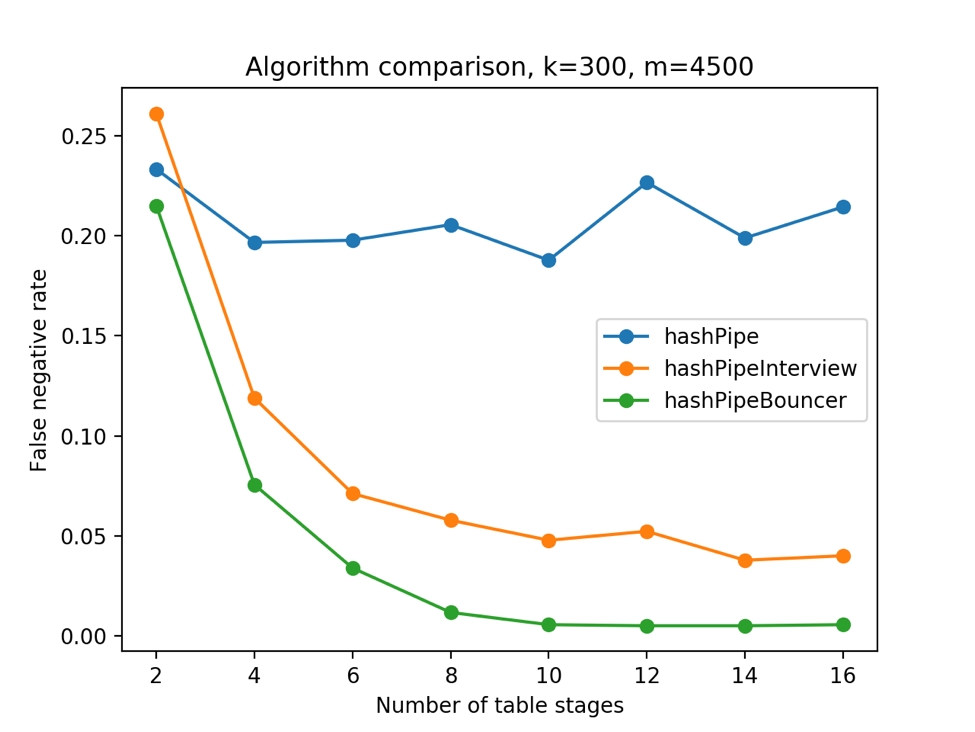
\includegraphics[scale=0.5]{stageComparison}
     \caption{Comparison of algorithms when number of table stages is varied. Interview and Bouncer do not suffer from the same accuracy drawbacks as the baseline when increasing the number of table stages}
     \label{fig:bp-image}
\end{figure}

\begin{figure}[t]
  \centering
    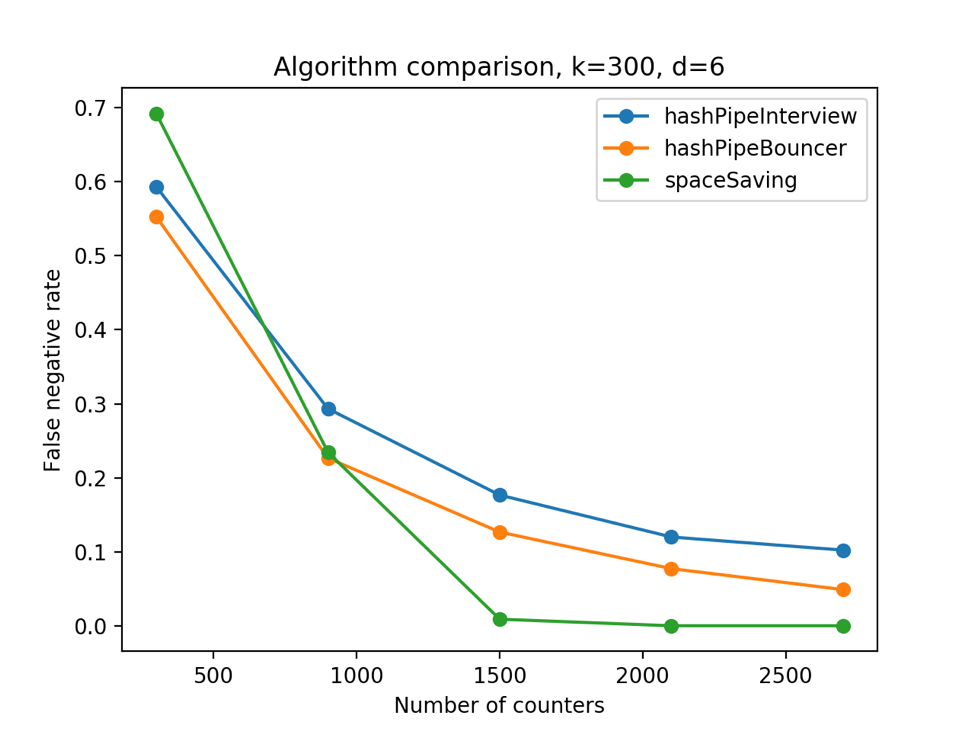
\includegraphics[scale=0.45]{spacesaver}
     \caption{Comparison of Interview and Bouncer with Space Saver}
     \label{fig:bp-image}
\end{figure}
\section{Related Work}
\label{sec:related}

\subsection{Sampling Algorithms}
Rather than count the frequency of each packet, one family of heavy hitter algorithms is based on infrequent sampling. While this approach improves scalability and drastically reduces memory usage, sampling comes at the cost of decreased accuracy. The algorithms Sampled NetFlow and Sample and Hold follow this approach by sampling each packet with some very small probability, such as 0.1 percent or even 0.01 percent. Sample and Hold improves upon Netflow, since once a flow is sampled, a corresponding counter is held in a hash table in flow memory until the end of the measurement interval. The entry for a flow is updated for every subsequent packet belonging to the flow. According to this scheme, the error is proportional to 1/M, as opposed to 1/Mfor a classical sampling algorithm, where M is the available memory. 

\subsection{Sketch Algorithms}
Sketch algorithms are a family of algorithms that attempt to answer questions about data streams by leveraging approximation. By sacrificing accuracy, sketch algorithms allow the heavy hitter problem to be tackled using a limited amount of memory. One of the most prominent of these algorithms is Count-Min Sketch, which uses a two-dimensional hash table to approximate counts. Each packet is hashed using d different hash functions, and the counter in each of the d corresponding buckets is incremented. Hash collisions will cause certain bucket counts to be incremented for different flow identifiers, so to approximate the count for a given identifier, it is hashed using the d hash functions, and the minimum of these bucket counts it used. This method is hardware-friendly, but sketch based algorithms do not track the flow identifiers associated with each count, so reporting the frequency of the top k flows is not accurate.

\subsection{Counter Based Algorithms}
Counter Based Algorithms process every flow, but due to memory constraints, are only able to maintain a counter of a constant number of the heaviest flows. Therefore, these algorithms aim to retain counters of only heavy hitters while ignoring lighter flows through the use of strategic admission and eviction policies. Space Saving maintains a table of the frequencies of N flows, evicting the least frequent flow each time an unmonitored flow is encountered. The newly admitted element assumes the frequency of the evicted flow. This eviction policy results in large errors for heavy-tailed workloads, where many new small flows may wrongly evict larger flows. Furthermore, depending on the hardware implementation, it may be resource intensive to find the least frequent flow in the table for every newly encountered flow. 
The intuition behind Randomized Admission Policy (RAP) is to minimize this error by being much more conservative about the elements that are admitted into the table. Instead of evicting the minimum element in the table for every new flow encountered, RAP only admits new flows with a probability of $1/(c_m + 1)$, where $c_m$ is the minimal counter value. By being more conservative, RAP has increased accuracy over Space Saver, but also makes it more difficult for new larger flows to gain admission. In our approach, we adopt elements of the randomized admission policy to prevent false evictions while also dampening the adverse effects of a conservative policy. 

\begin{figure}[t]
  \centering
    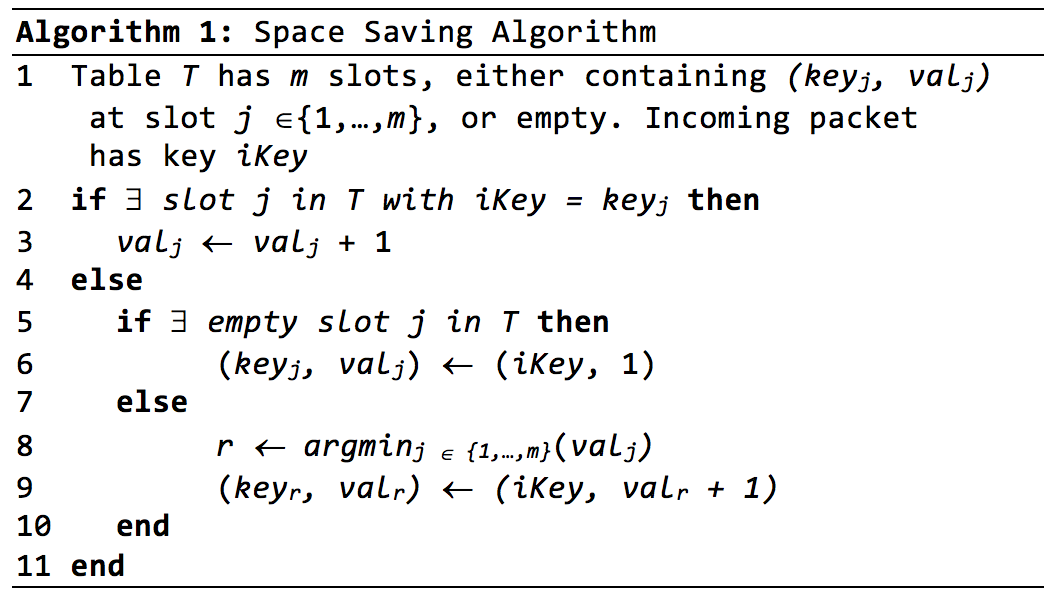
\includegraphics[scale=0.5]{alg1}
     \label{fig:bp-image}
\end{figure}

HashPipe is heavily inspired by Space Saver, but leverages feed-forward packet processing to divide the task of finding the minimum into small parts. The algorithm consists of d stages, each with its own hash function hd and an associated hash table. When a packet enters the pipeline at the first stage, the hash function h0 is used to hash its identifier to a bucket. Each bucket will contain a flow identifier and its associated count. If the identifier of an incoming packet matches the identifier stored in the bucket it hashes to, the count is incremented, and no further processing is done. Similarly, if the bucket is empty, the identifier is added with a count of 1, and processing stops. However, the rest of the pipeline comes into play if the incoming packet identifier does not match the stored packet identifier. In this case, the stored packet will be evicted, and the incoming packet will be stored in its place with a count of 1. In actual implementations of HashPipe on hardware, the identifier and count of the “evicted” packet is added to the incoming packet as metadata, and the original packet continues to flow down the pipeline with this metadata.

\begin{figure}[t]
  \centering
    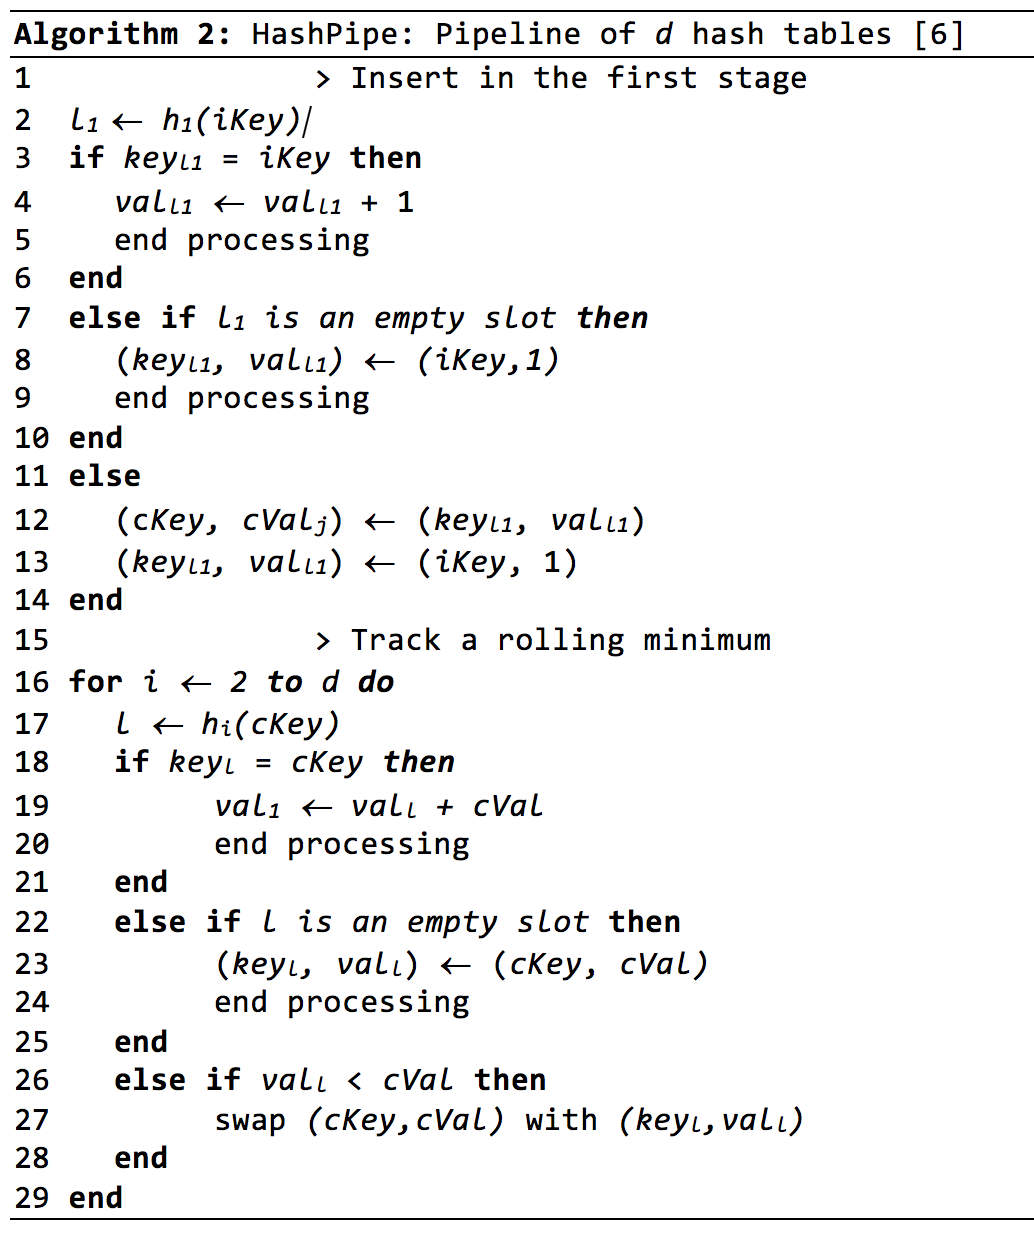
\includegraphics[scale=0.42]{alg2}
     \label{fig:bp-image}
\end{figure}

In subsequent stages, the key-counter pair that has been evicted is hashed using the corresponding hash function hd and it is compared to the stored value in that bucket. Instead of always evicting like in the first stage, the stored value will only be evicted if it is the minimum between the two counter values. If the stored value is less, the key-counter pairs are swapped, and the key previously in the table becomes the carried key. This same process is repeated at each stage until one pseudo-minimum value is carried off the end.

Instead of attempting to find a true minimum, as is the case in Space Saver, HashPipe settles for a probabilistic minimum, obtained by comparing only one value per stage. The main idea behind the pipeline is that heavy flows will be retained and lighter flows will be evicted over time. HashPipe is useful because for each packet, there is only one read per table. This allows for efficient stream processing and gets around hardware constraints that do not allow multiple reads to the same table. The downside of this scheme is that it does not prevent duplicate keys across different tables. When a count is stored for the same keys in different stages, this reduces the space available to hold onto heavier flows. However, duplicates have been shown to account for only 5-10 percent of table space, and have a limited impact on accuracy [CITATION]. With a fixed amount of memory available to the hardware, the number of stages d can be tuned: a greater number of stages increases heavy flow retention because more slots are sampled to pick a minimum, but it will increase the number of duplicates.
\section{Conclusions}
\label{sec:conclusion}

We set out to create an algorithm that solves the top-$k$ Heavy Hitters problem while making efficient use of switch hardware functionality. Building off of HashPipe, we created an algorithm, HashFilter, with two variants of restricted admission policy: Bouncer and Interview. These achieved the same accuracy of HashPipe while requiring less than half of the memory resources. Using real traffic data, we show experimental results that justify our design choices and prototype HashFilter with P4 to confirm its viability on hardware.

%% Bibliography
%\vspace{-1ex}
%\linespread{1.0}
%\setlength{\bibsep}{1pt}
%\footnotesize
\small
\bibliography{local}
\bibliographystyle{abbrvnat}

\end{document}

